\documentclass{article}
\usepackage[utf8]{inputenc}
\usepackage[T1]{fontenc}
\usepackage{graphicx}
\usepackage{hyperref}
\usepackage{geometry}
\geometry{margin=1in}

\title{ESCAMADE}
\date{Encyclopaedia Britannica (1771)}

\begin{document}
\maketitle

\section*{Historical source}
\textbf{Entry ID:} \texttt{entry-escamade-1473} \\
\textbf{Volume ID:} 149979622 \\
\textbf{Character Count:} 1296

\subsection*{Extracted Text}
ESCAMADE, or Sealana a farism attack of a
wall on a rampart; carnivore with ladders, to pafs the
ditch or mount the rampart; without proceeding in
forsp, breaking ground, or carrying on regular works
of feature the menu.

When an throws are prepared to pafs the ditch,
clicks with the affilance of bounds, humble, and life
cines, when it is muddy, or with fault boats of tin, or
baskets covered with films or collected, where it is deep
and filled with water, a party must be placed on the
counterfeary opposite for the loading-place, ready to
fire at the garden if they are alarmed, and good the
mounting on the rampart. It the ditch is dry, the
ladders so fixed in Some place fartheit diflant from the
century and a four as they get upon the rampart
they put themforce in order to reverse the enemy; if
the country should be farparified and likely overcome,
the attachments halten to break open the gate and to
let in the raft of the party. If lifted this is wet, the
rampart high, and provided with a reverentes, it will
he difficult to impute the town in the way; but if
there is no economic, the troops may hide chambers
along the outside of the rampart till all are over. Since the invention and use of gunpowder, and the
walls of cities have been linked, they are foldom taken
by efcalade.



\section*{Source record}
\begin{itemize}
\item \textbf{Dataset:} \texttt{NationalLibraryOfScotland/encyclopaedia\_britannica\_illustrated}
\item \textbf{Dataset Revision:} \texttt{309f765b1ecc83e0a7f7762e44b4a927a7555443}
\item \textbf{Page ID:} \texttt{britannica:309f765b1ecc83e0a7f7762e44b4a927a7555443:train:1473} \\
  \textbf{Filename:} \texttt{page-1473-b3b602ef6a3d.jpg} \\
  \textbf{Row Index:} 1473 \\
  \textbf{SHA256:} \texttt{b3b602ef6a3d4961...}
\end{itemize}

\begin{figure}[h]
\centering
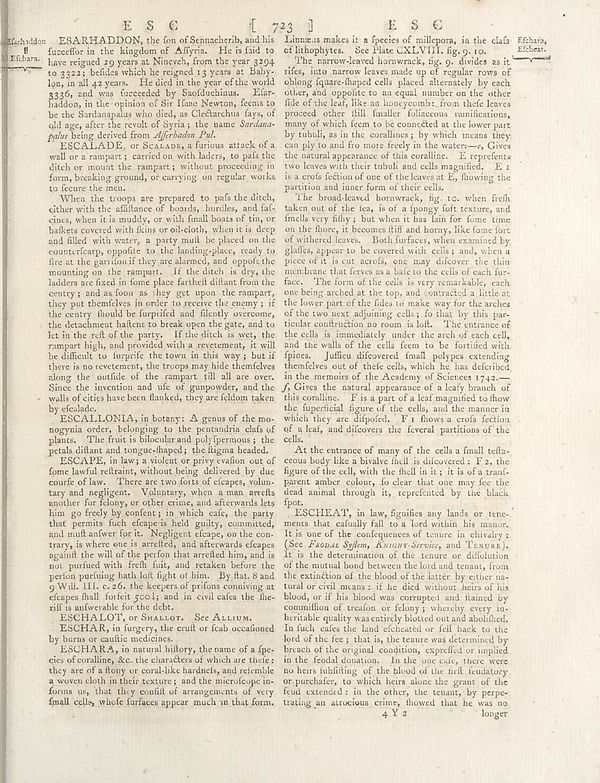
\includegraphics[width=0.85\textwidth]{../scans/page-1473-b3b602ef6a3d.jpg}
\caption*{Source scan: \texttt{page-1473-b3b602ef6a3d.jpg}}
\end{figure}

\end{document}
